We use $\bar{x}=[x_1, \ldots, x_n]$ to represent a list of values, and $\bar{x}_1:\bar{x}_2$ to represent the concatenation of $\bar{x}_1$ and $\bar{x}_2$.
$f(\bar{x}) = [f(x_1, c), \ldots, f(x_n, c)]$. $s_0 \oplus \bar{x} = \textit{reduce} \ s_0\  \bar{x}$ where $s_0$ and $\oplus$ are as defined in section \ref{sec1}.

\subsection{Motivations}

\textbf{Blocked execution of a single \textit{broadcast-and-then-aggregate}}.
When the input list $\bar{x}$ is too large to be processed within hardware constraints,
We need to split it into portions that can be handled by the hardware.
By definition, the \textit{broadcast-and-then-aggregate} operation can be executed portion by portion. This means that the following equation holds:

\begin{equation}
s_0 \oplus f(\bar{x},c) = \left(s_0 \oplus f(\bar{x}_1,c)\right) \oplus \left(s_0 \oplus f(\bar{x}_2,c)\right)\ \ \ \text{where}\ \ \bar{x} = \bar{x}_1 : \bar{x}_2
\end{equation}

Assuming that the input list $\bar{x}$ is divided into two segments, $\bar{x}_1$ and $\bar{x}_2$, the broadcast stage can independently evaluate the function $f$ on each segment.
This results in $\bar{y}_1 = f(\bar{x}_1,c)$ and $\bar{y}_2 = f(\bar{x}_2,c)$, which can be executed in parallel.
The reduce operation is recursively defined and aggregates each segment independently to obtain partial aggregated results.
For example, $s_1 = s_0 \oplus \bar{y}_1$ and $s_2 = s_0 \oplus \bar{y}_2$.
These partial results are then recursively combined until a single aggregated value is obtained, such as $s = s_1 \oplus s_2$.
\textbf{\textit{If the operator $\oplus$ is both associative and commutative, the partial reduction can be computed in parallel}}.

Regarding a single \textit{broadcast-and-then-aggregate} operation, the final aggregated result depends on completing the scan of all the list inputs.
This makes the reduce operation a barrier to proceeding further.
Furthermore, if the output of the broadcast stage is required for subsequent computations,
it must be stored in memory. This requires storage proportional to the length of the input sequence.

\textbf{Motivations for blocked execution for a chain of \textit{map-and-then-aggregate} operations}.
If the input list is very long, the time it takes to scan the input and write the results of the broadcast stage (if needed) will be the dominant factor in the overall latency of the \textit{map-and-then-aggregate} operation.

If the entire computational process can be executed in parallel, with each portion computing a partial result,
an efficient implementation can exploit the memory hierarchy by caching segments of input list in high-speed memory.
Computation can then continue in high-speed memory until a synchronization barrier is met, at which point partial results must be stored in slow memory.

In the \textit{broadcast-and-then-aggregate} operation, the \textit{broadcast} stage requires storage proportional to the length of the input to store its output,
while the \textit{reduce} operation aggregates input to a smaller value that consumes less storage for its output.
If a chain of \textit{broadcast-and-then-aggregate} can proceed portion by portion in high-speed memory until the results of the broastcast stage are no longer needed by subsequent computation (and therefore do not need to be stored),
both I/O complexity and memory footprint can be reduced.

We use the attention example shown in Figure \ref{attn} as our running example. 
There are three \textit{broadcast-and-then-aggregate} operations involved.
Each can execute internally in parallel, block by block.
However, the three \textit{broadcast-and-then-aggregate} operations must execute sequentially since there are data dependences among them.
Additionally, the result of the first broadcast operation is required by the second broadcast operation, and the results of the second broadcast operation are required by the third broadcast operation.
Sequentially execute these three \textit{broadcast-and-then-aggregate} requires two storages that are proportional to the input list.

\lstset{
  frame=lrtb,
  backgroundcolor=\color{aliceblue},
  numbers=left,
  numbersep=1em,
  xleftmargin=1em,
  breaklines=true,
  linewidth=\linewidth
}
\begin{lstlisting}[language=code_example2, caption={}]
// stage1: local reducer computes partial results on individual blocks
(:$o_1$:) = Attention((:$q, ks_1, vs_1$:))     (:$o_2$:) = Attention((:$q, ks_2, vs_2$:))

// stage2: combine partial results
(:$o_{\text{new}}=\text{Combiner}(o_1,o_2)$:)
\end{lstlisting}

After the last \textit{broadcast-and-then-aggregate} operation, a noticeable decrease in storage size was observed.
Therefore, we anticipate that the entire computational process of equation (\ref{eq::attn}) be executed in two stages.
In the first stage, the input will be split into portions and partial results that require storage much smaller than the original input list will be computed without regard to original data dependencies among dependent \textit{broadcast-and-then-reduce} operations.
By selecting an appropriate block size, the entire computational process can be stored in high-speed memory.
In the second stage, a combiner will merge these partial results to obtain the correct final aggregated value.

The problems are:
\textcolor{red}{
\begin{enumerate}
    \item Under what conditions (necessary and sufficient conditions) can dependent \textit{broadcast-and-then-aggregate} operations be decomposed into these two stages?
    \item The existence of a combiner that can compute the correct final result.
    \item If such a combiner exists, how can it be constructed?
\end{enumerate}
}

\subsection{A (informal) Problem Statement}

Given two dependent \textit{broadcast-and-then-aggregate} operations:
\begin{align*}
    r &= s_0 \oplus_1 f_1(\bar{x} - c) \\
    o &= s_1 \oplus_2 f_2(\bar{y} - r)
\end{align*}

Design a combiner, denoted by $C$, that can produce an output $\Bar{\Bar{o}}$ equivalent to $o$ when computed using the following formula:
    
\begin{align*}
    r_1 &= s_0 \oplus_1 f_1(\bar{x}_1,c) && r_2 = s_0 \oplus_1 f_1(\bar{x}_2,c) \\
    o_1 &= s_1 \oplus_2 f_2(\bar{y}_1,r_1) && o_2 = s_1 \oplus_2 f_2(\bar{y}_2,r_2) \\
    \Bar{\Bar{o}} &= C(r_1, r_2, o_1, o_2)
\end{align*}

Note that a combiner $C(r_1, \bar{y}_1, r_2, \bar{y}_2)$ always exists.
This is because $r$ can be computed as $r = r_1 \oplus r_2$, and then $o$ can be re-computed using the formula $o = s_1 \oplus_2 f_2(\bar{y}_1:\bar{y}_2, r)$. 
However, implementing such a combiner would require storing the entire $\bar{y}$ and re-computing the second \textit{broadcast-and-aggregate},
which is not practical.

In order to reduce both IO complexity and the storage requirements, we must ensure that the combiners only depend on the outputs of the \textit{reduce} operations, namely $r_1$, $r_2$, $o_1$, and $o_2$.

\subsection{Preliminary Thinking to the Problem}

\textit{\textcolor{red}{Decomposable Broadcast-and-then-Aggregate Operation}}.
% A broadcast operation $F$ is decomposable under $g$ if there exists a function $h$ such that $F(x, g(c,\triangle c))=F(F(x, c), h(c,\triangle c))$.
% A decomposable broadcast $F$ under $h$ allows you broadcast the value $g(c, \triangle c)$ in two broadcast operations: first broadcast $c$ using $F$, and then broadcast an adjusting fanctor $h(c, \triangle c)$ using $F$.
We say that a \textit{broadcast-and-then-aggregate} operation $R=<F,c,s_0,\oplus>$ is decomposable under $\circ$ if there exists functions $h$ and $\odot$ such that the following equation holds:

\begin{equation}
s_0 \oplus F(\bar{x}, c \circ \triangle c)=(s_0 \oplus F(\bar{x}, c)) \odot h(c, \triangle c)\label{conds}
\end{equation}

In other words, a decomposable \textit{broadcast-and-then-aggregate} allows to broadcast a value $c \circ \triangle c$ in two steps.
First, broadcast $c$ to the input list using $F$, and then aggregate the broadcast result using $\oplus$.
Second, adjust the result of the first step with an adjusting function $h(c, \triangle c)$ using $\odot$.

% \noindent \textbf{Some examples}.

% $f(\bar{x}+c) = \bar{x} + c$ is decomposable under $+$: $f(\bar{x}+(c+\triangle c))=f(\bar{x}+c)+n\triangle c$, where $g(c, \triangle c)=n\triangle c$.
% It is also decomposable under $*$: $f(\bar{x}+c*\triangle c) = f(\bar{x~}+c) + (c * \triangle c - c)$.

% $f(\bar{x},c) = \log(c*\bar{x})$ is decomposable under $*$, but $f(\bar{x},c) = \log(c+\bar{x})$ is not decomposable under $+$.

If a \textit{broadcast-and-then-aggregate} operation can be decomposed, then a combiner $C$ exists by the definition.
Since this definitive equation(\ref{conds}) is a strict necessary condition,
and the problem is then reduced to determining the existence of the functions $\circ$ and $h$.
Unfortunately, it is easy to find counterexamples that demonstrate the non-existence of $\circ$ and $h$ for arbitrary $F$ in general case.

% \begin{align*}
%     r_1 &= s_0 \oplus_1 f_1(\bar{x}_1,c) && r_2 = s_0 \oplus_1 f_1(\bar{x}_2,c) \\
%     o_1 &= s_1 \oplus_2 f_2(\bar{y}_1,r_1) && o_2 = s_1 \oplus_2 f_2(\bar{y}_2,r_2) \\
% \end{align*}

% A correct aggregated value of the first \textit{broadcast-and-then-aggregate} can be obtained simply using: $r'= r_1 \oplus_1 r_2$.
% And the second \textit{broadcast-and-then-aggregate} should be re-computed.

% \begin{align*}
% f_1(\bar{y}_1, r') = f_1(\bar{y}_1, \textcolor{red}{h}(r_1, \triangle r_1)) = f_1(\bar{y}_1,r_1)
% \end{align*}

% Denote $\triangle r_1 := h(r', r_1)$ and $\triangle r_2 := h(r', r_2)$.
% We then re-compute the second \textit{broadcast-and-then-aggregate}:

% $f_2(\bar{y}_1, r_1 \circ \triangle r_1) = f_2(\bar{y}_1,r_1) \triangle r_1, h(r', r_1)) = f_2()$

% % \triangle r_1 &= \textcolor{red}{h}(r', r_1) && \triangle r_2 = \textcolor{red}{h}(r', r_2)\\
% % o_1 &= \\
% % \Bar{\Bar{o}} &= C(r_1, r_2, o_1, o_2)

% Given the dataflow graph Figure \ref{fused-map-and-aggreage}, let's go through flash attention step by step.
% The problem is, given partial results: $m_1$, $m_2$, $d_1$, $d_2$, $o_1$ and $o_2$, construct three combiners: $m = C_1(m_1, m_2)$, $d = C_2(m_1, m_2, d_1, d_2)$ and $o = C_3( m_1, m_2, d_1, d_2, o_1, o_2)$ to obtain an aggregated results.

% This is what flash attention does to the original attention computation.
% Figure \ref{fused-map-and-aggreage} virtualizes this process.

\begin{figure}[h]
    \centering
    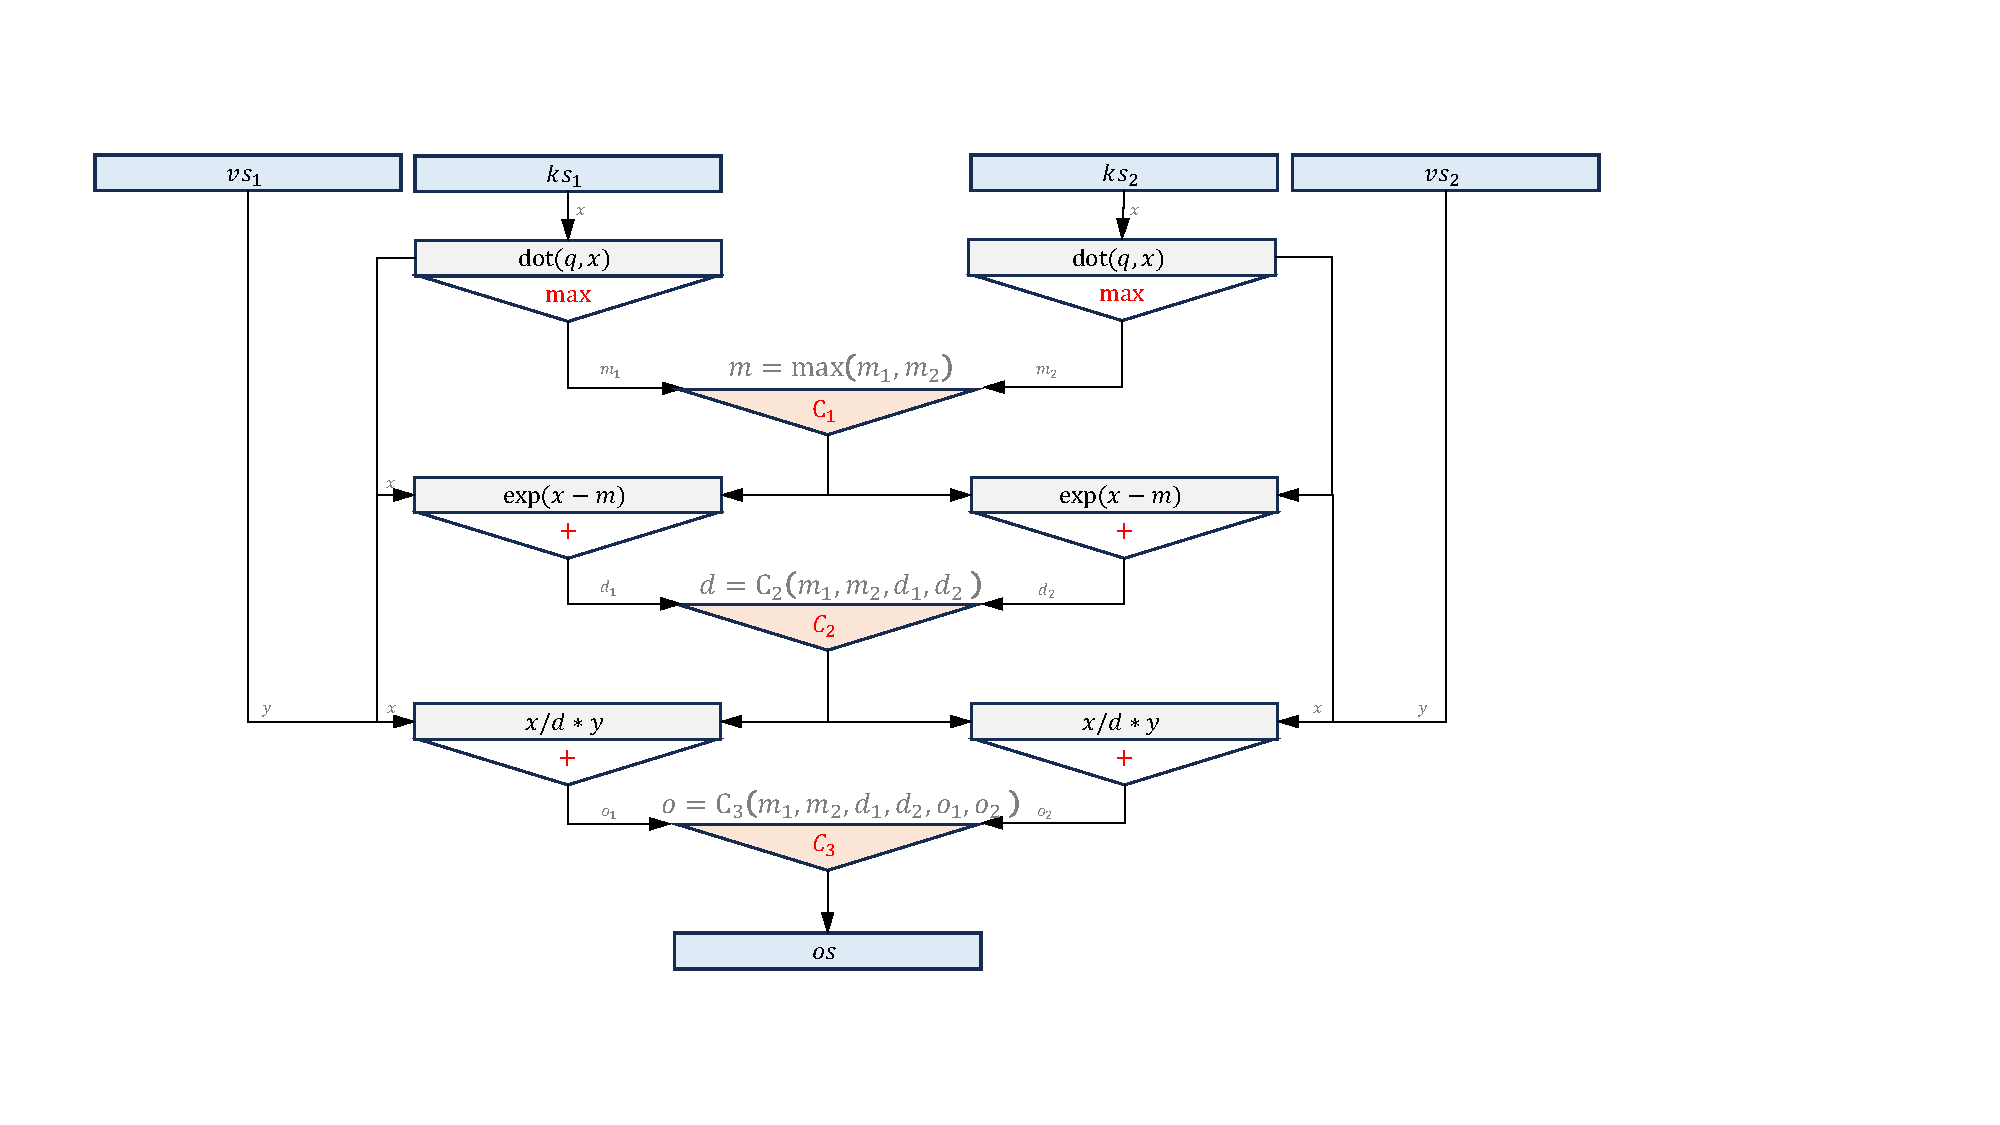
\includegraphics[width=1\textwidth]{figures/attention_expression_tree2.pdf}
    \caption{The expected blocked execution of a chain of \textit{Broadcast-and-then-aggregate}s.} \label{fused-map-and-aggreage}
\end{figure}

In the particular instance of flash attention, a combiner exists.

\colorbox{NavajoWhite}{For the first \textit{BroadcastAndThenAggregate}}, $C_1$ is trivial that is equal to the original reduce function: $m = C_1(m_1, m_2) = \max(m_1, m_2)$.

\colorbox{NavajoWhite}{For the second instance of \textit{BroadcastAndThenAggregate}}, consider the following sub-problem:
$\bar{y}_1=\exp(\bar{x}-m_1)$ has been computed for a single block,
but a new constant factor $m$ needs to be broadcast for the entire list.
This requires re-computing $\bar{y}_1' = \exp(\bar{x}-m)$.
The solution is to recover $\bar{x}$ from $\bar{y}_1$ and $m_1$ by computing: $$\bar{x}= \log(\bar{y}_1) + m_1$$

then substitue $\bar{x}$ into the equation that computes $\bar{y}_1'$. That is:

\begin{align*}
\bar{y}_1' &= \exp\left(\log \left(\bar{y}_1\right) + m_1 -m \right) \\
&= \bar{y}_1\exp(m_1 - m)
\end{align*}

Therefore:
\begin{enumerate}
\item the updating euqation for the broadcast step is: $\bar{y}_{\text{new}}=\bar{y}_{\text{old}}\exp(m_\text{old}-m_{\text{new}})$
\item combine partial results: 
\begin{align*}
   d=&C_2(d_1,d_2) = d_1 * \exp(\triangle m_1) + d_2 * \exp(\triangle m_2) \\
   \triangle m_1 :=&m_1 - \max(m_1, m_2) \\
   \triangle m_2 :=&m_2 -\max(m_1, m_2) \\
\end{align*}
\end{enumerate}

\colorbox{NavajoWhite}{For the third instance of \textit{BroadcastAndThenAggregate}}, consider the following sub-problem:
$\bar{o}_1=\frac{\bar{x}_1}{d_1}*\bar{y}$ has been computed for a single block,
but a new constant factor $d_2$ needs to be broadcast for the entire list.
This requires re-computing $\bar{o}_1' = \frac{\bar{x}_1'}{d}*\bar{y}$.
The solution is to recover $\bar{x}_1*\bar{y}$ from $\bar{o}_1$ and $d_1$ by computing: $$\bar{x}'_1 * \bar{y}= \exp(\triangle m_1)*\bar{o}_1 * d_1$$

Then the adjusted $o_1'=\frac{\exp(\triangle m_1)*o_1*d_1}{d} = o_1 *\frac{d_1 \exp({\triangle m_1})}{d_1 * \exp(\triangle m_1) + d_2 * \exp(\triangle m_2)}$, and $o = C_3(o_1, o_2) = o_1 * \frac{d_1 * \exp(\triangle m_1)}{d_1 * \exp(\triangle m_1) + d_2 * \exp(\triangle m_2)} + o_2 * \frac{d_2*\exp(\triangle m_2)}{d_1 * \exp(\triangle m_1) + d_2 * \exp(\triangle m_2)}$.


\subsection{A Counter-example: Logsoftmax instead of softmax}

\begin{figure}[h]
    \centering
    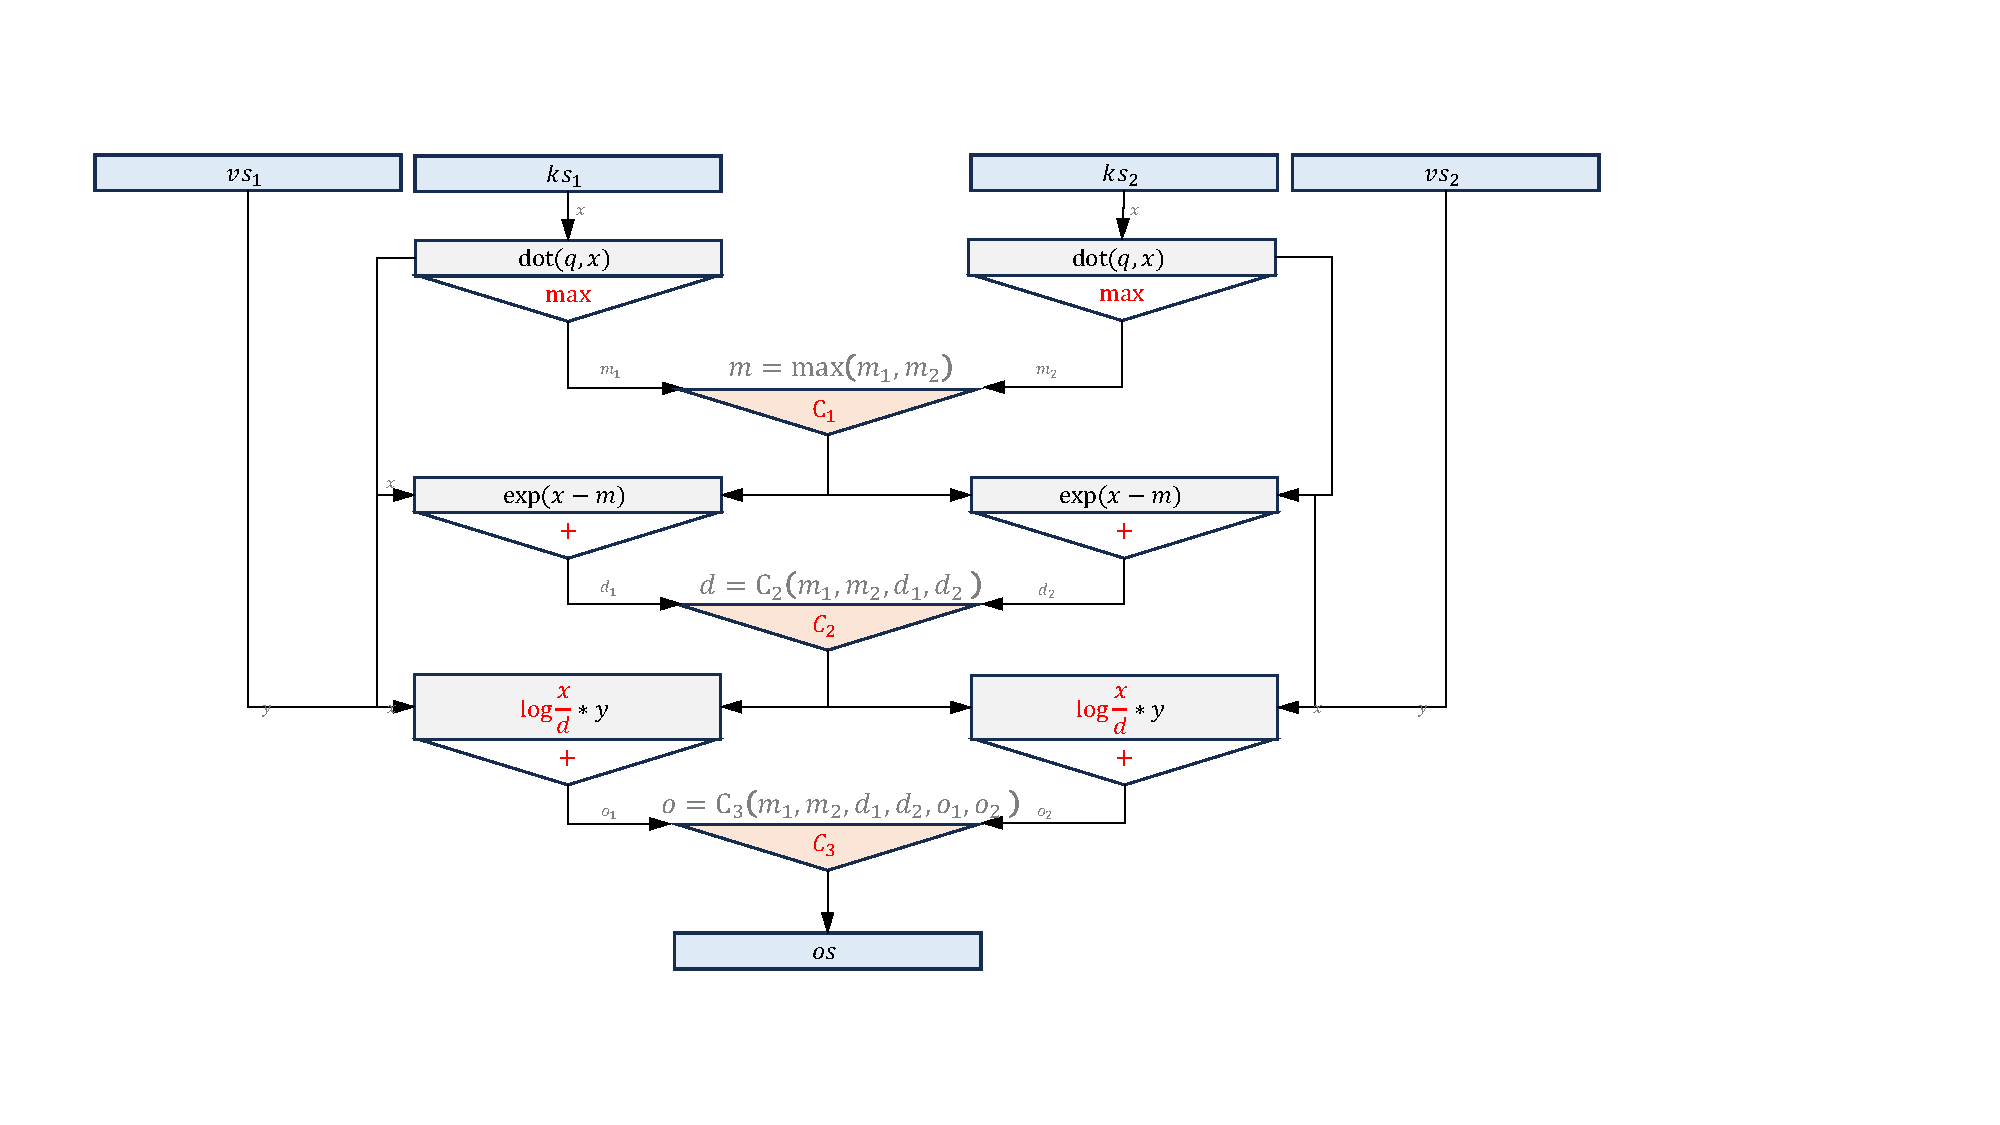
\includegraphics[width=1\textwidth]{figures/attention_expression_tree3.pdf}
    \caption{An imaginary example: use logsoftmax instead of softmax.}
\end{figure}

Let's think of an imaginary example, that compute:

$$\text{Attention}(Q, K, V) = \text{logsoftmax}(QK^T)V$$

$C_1$ and $C_2$ doest not change, thus: how $C_3$ looks like.

Suppose $\bar{z}_1$ and $o_1$ are results for the broadcast stage, and reduce stage computed on input blocks $\bar{x}_1$ and $\bar{y}$ respectively:
\begin{align*}
\bar{z}_1 &= \log\left(\frac{\bar{x}_1}{d_1}\right)*\bar{y} = \bar{y}*\log(\bar{x}_1) -\bar{y}\log d_1\\
o_1 &= \sum(0, \bar{z}_1)
\end{align*}

Then it is required to compute an updated $\bar{z}_1'$ and $o_1'$ since $\bar{x}_1$ and $d_1$ are updated.

We have:
\begin{align*}
    \bar{z}_1'&=\log \left(\frac{\bar{x}_1'}{d}\right) * \bar{y} = \bar{y}\log\bar{x}_1' - \bar{y}\log d \\
    \bar{x}_1' &= \exp(m_1 - m)\bar{x}_1 \\
    d &= \exp(m_1 -m)d_1 + \exp(m_2 -m)d_2
\end{align*}

Thus we have:
\begin{align*}
\bar{z}_1'&=\bar{y}\log\left(\exp(m_1-m)\bar{x}_1\right) - \bar{y}\log{d} \\
&=\bar{y}\left((m_1-m)+\log(\bar{x}_1)\right) -\bar{y}\log d \\
&=\bar{y}(m_1-m-\log d)+\bar{y}\log(\bar{x}) \\
&=\bar{y}(m_1-m-\log d)+\bar{z}_1+\bar{y}\log d_1 \\
&= \bar{y}(m_1-m-\log d+\log d_1)+\bar{z}_1
\end{align*}

Given $\bar{z}_1'$:
\begin{align*}
    o_1'&=\text{sum}(0, \bar{z}_1') \\
    &=(m_1-m-\log d+\log d_1)\text{sum}(0, \bar{y}) + o_1
\end{align*}

Update $o_1$ has to access its input $\bar{y}$ and compute an extra reduction sum on it.